\chapter{Олег}

Когда и где родился Олег, прозванный не то Греками, не то киевлянами, Вещим? Летописи молчат.

Он возникает на страницах летописей совместно с Рюриком, Синеусом и Трувором. Об Олеге сказано: «племянник Рюрика», «сродник Рюрика», «племянник воевода Рюрика Олег». В Иоакимовской летописи Олег – шурин Рюрика, князь Урманский. Татищев упоминает также о раскольничьей рукописи, где Олег – вуй Ингоря, то есть брат его матери. Но Татищев приводит выдержку из другого источника, где Олег уже дядя Ингоря, брат отца. Ах, если бы видеть те источники, на которые ссылался Татищев!

У Гилярова\cite[стр. 212]{gilyarov01} есть очень любопытный в смысле именований текст, хотя эдак века 16-го или позже:

\begin{quotation}
Игорь же или георг петинадесят лет остав по отце единовладетеле, тщанием олехны, князя олехнанского, дяди своего, его же потом воеводу себе постави, черкасы, крымляны, печенеги, нагайцы, донцы и своевольные запорожаны (идеже ныне казаки), се есть малую тартарию, покоря и самаго царя константинополскаго дань даяти принуди; потом толико щасливыи победитель в седние века мальдитом князем, данником, наследником дыровым, древлянским государем, убиен бысть.
\end{quotation}

Князь Олехна. Мальдит вместо привычного «Мала», да еще наследник Дира – Дыра. Олехна назван дядей Игоря. Но в других списках Олег – племянник Рюрика. Раз племянник, то Игорю он – двоюродный брат. Если по смерти Рюрика Игорю было не пару лет, а пятнадцать, то разница возрастов между Олегом и Игорем не так уж велика.

%или В\'олха

О молодом Олеге находим много любопытного в былинах. По ним, отцом Вольг\'и был змей, изнасиловавший будущую мать богатыря. Змей это не рептилия, а бес, черт, один из тех, кого погане почитали за богов, и кого после принятия христианства начали именовать бесами и змеями. В некоторых былинах змей, отец Вольги, именован змеем Горынычем. Вольга – полукровка, человек лишь наполовину.

Он развивается быстрее, чем другие дети – умственно и физически\cite[стр. 1]{rybnikov01}:

\settowidth{\versewidth}{Пошел Вольга сударь Буслаевичь по сырой земли:} 
\begin{verse}[\versewidth]
Рос Вольга Буслаевичь до пяти годков,\\
Пошел Вольга сударь Буслаевичь по сырой земли:\\
Мать сыра земля сколыбалася,\\
И звери в лесах разбежалися,\\
И птицы по подоблачью разлеталися,\\
И рыбы по синю морю разметалися.\\
И пошел Вольга сударь Буслаевичь\\
Обучаться всяких хитростей, мудростей,\\
И всяких языков разныих;\\
Задался Вольга сударь Буслаевич на семь год,\\
А прожил двенадцать лет;
\end{verse}

Числа в былинах разнятся – то Вольга в пять лет постигает все мудрости, то в семь. В семь лет он уже как двенадцатилетний. А к семнадцати годам уже собирает дружину, сам величается атаманом.

Мне вспоминается «Мабиногион», сборник уэльских легенд 11-12 веков. Одна из них называется «Пуйшт, король Дэведа» (Pwyll prince of Dyved) – имена на русском пишу так, как они произносятся на среднеуэлльском. У Пуйшта была жена, Рхианнон – из народа фэйри (fairy). Фэйри, более привычные нашему читателю как «феи» – они ведь без крылышек были. Фэйри, эльфы, альвы были для христиан тем же, что языческие божества на христианской Руси – демонами.

У Пуйшта и Рианнон родился сын Гури Вашт Эйрин (Gwri Wallt Euryn, Gwri Золотоволосый), полу-фэйри. Его похищают, он попадает к приемным родителям\cite{mabinogion}:

\begin{quotation}
[...] и они окрестили мальчика, и обряд был проведен там; и имя которое они ему дали было Гури Вашт Эйрин, потому что волосы на его голове были желты как золото. И они растили мальчика во Дворе, пока ему не исполнился год. И до того, как год закончился, он мог уверенно ходить. И он был больше, чем мальчик трех лет отроду, даже самый крупный и сильный. И мальчик воспитывался второй год, он был большой, как шестилетний. И до того, как завершился шестой год, он подкупал конюхов, чтобы те позволяли ему водить лошадей на водопой.
\end{quotation}

Ничего не напоминает?

Нет, я не отождествляю Вольгу с Гури Ваштом Эйрином. Но я вижу чрезвычайное сходство развития двух полукровок, детей человеческих и \textit{других}, к тому же вероятно как-то связанных с иным течением времени.

Подобное раннее развитие имеет и ирландский «народный герой» Кухулин, тоже полукровка, сын обычной женщины и Луга (рожденного от принцессы-фомойри и мужчины из числа Туаха Дэ Дананн). Грубо говоря, Кухулин был полуэльфом.

Тут нам снова придется немного коснуться ирландских легенд. Точнее, того глубинного слоя ирландской истории, который принимается наукой за сказочный и отбрасывается. 

Если не отбрасывать, то летописание Ирландии выглядит так. Вначале людей обычных там вообще нет. Ирландию делят народы Фир Болг, Фомойри, и Туаха Дэ Дананн. Фир Болг – обитатели пещер. Фомойри выглядели по-разному. Одни были вполне как люди, причем невиданной красоты. Другие – козлоголовые. Третьи – с одним глазом, одной рукой и ногой\footnote{Подобных встречаем в преданиях якутов.}. Туаха Дэ Дананн прибыли в Ирландию и сожгли за собой корабли. Явились в черных тучах и высадились в горах Conmaicne Rein в Connacht. Три дня не было видно солнца.

Туаха Дэ Дананн сосуществовали и воевали с Фир Болг, Фомойри, позже были вытеснены людьми из клана Мила Испанского и постепенно ушли в эдакое подполье, сделав словно невидимыми себя и свои жилища. Туаха Дэ Дананн стали теми, кого называют «фэйри», «эльфы» или «хулдуфолк» (у исландцев). Некоторые поздние предания смешивают Туаха Дэ Дананн и Фомойри – а впрочем они сами смешивались, и рождались у них дети.

Незримые жилища поначалу Фомойри, а затем и Туаха Дэ Дананн называли «ши» (пишется Sidhe – что значит «крепость фэйри»), а жителей их именуют áes sídhe, то есть «народ ши», либо сокращенно «ши»\footnote{Отсюда например известное слово «банши» – bean sidhe.}. В русских переводах зачастую вместо «ши» встречается слово «сид».

Местности ши, насколько я понимаю, находятся в некоем «другом мире», но в координатной системе привычного нам мира. Например, там где для людей – какие-то развалины, для фэйри – дворец. Такими ши считаются и некоторые холмы\footnote{Подобным образом в преданиях Урала, Сибири уходит подобная эльфам Чудь белоглазая – внутрь гор ли, под землю или в другой мир – осмысление перехода, или исхода, ускользает от человеческих повествователей.}. Иногда фэйри покидают другой мир (или режим бытия) и живут среди людей. Время в мире эльфов течет медленней, чем в нашем. Попав туда на пару дней и вернувшись сюда, человек обнаруживает, что прошло много лет. Это неким образом связано с ускоренным развитием здесь, в нашем мире, детей, в ком течет «тамошняя» кровь.

Так вот, в повествовании «Битва при Маг Тьюирэд» (Cath Maige Tuired) есть герой, король Ирландии по имени Брес (Bres)\footnote{Сходство с «берестой», конечно же случайно.}. Он – сын златовласого Фомойри, принца  Элаты (Elatha), и Эри (Eri), что из Туаха Дэ Дананн. Во «Второй битве при Маг Тьюирэд» описано рождение Брэса\cite{cathmaigetuired}:

\begin{quotation}
Затем она родила мальчика и назвала его Eochu Bres, как хотел Элата. Через неделю после рождения он вырос как за две; и продолжал быстро расти семь лет, пока не стал ростом как 14-летний.
\end{quotation}

По преданию, Брэс был очень красивым, и в народе даже говорили «красив как Брэс». Но вернемся к Вольге!

Мать Вольги, согласно былинам – княжна Марфа Всеславьевна, проживающая в Киеве. Имена богатырских матерей в былинах подбирались, кажется, по красивости звучания.

Вольга былинный – оборотень, оборачивается в щуку чтобы плавать, в сокола – для полетов под облаками и достижения недоступных мест (например, чтобы подслушать разговор), волком – дабы рыскать во чистых полях. Этим способностям он стал учиться с десяти лет. И стал:

\settowidth{\versewidth}{Овернулся Вольга да малой птичиной,} 
\begin{verse}[\versewidth]
Птицей он летать да под оболоку\\
Рыбою ходить да в глубоки стана,\\
Зверями ходить да во темны леса.\\
Овернулся Вольга да малой птичиной,\\
Улетел-то Вольга да он под оболоку,\\
А й птицу всю да он порозгонял.
\end{verse}

И так далее. Сие воспринимается как сказка, ведь оборотничество в представлении современного читателя выглядит, наверное, как в кино, где герой, недоуменно уставившись на свои пальцы, рычит и обрастает шерстью. 

А давайте откроем теперь «Круг земной»\cite{snorry01} Снорри Стурлусона, где собраны различные предания исландцев. У скандинавов есть бог Один. Это бог смертный, точнее, обожествленный посмертно. Вот что говорится о нем, когда Один был живым:

\begin{quotation}
Один мог менять свое обличье. Тогда его тело лежало, как будто он спал или умер, а в это время он был птицей или зверем, рыбой или змеей и в одно мгновение переносился в далекие страны по своим делам или по делам других людей.
\end{quotation}

Пожалуй, нетрудно перебросить мосток к оборотничеству Вольги от этого описания трансового состояния с подключением сознания к чужому телу и управления оным.

Вероятно, состояние мнимой смерти и привело к поверью о живых мертвецах, ведь таковыми считались исключительно умершие ведьмы и упыри (ведьмачи). Глубокий транс, неотличимый от смерти, не мог быть распознан не то что селянами, но и опытными врачами – вспомним, как заживо похоронили Гоголя, хотя он завещал, чтобы тело предали земле только при появлении явных признаков разложения\footnote{Примечательно, что известный на землях Украины, можно сказать исторический упырь – Антоний Танский, являлся родичем Гоголя. У Антония Михайловича Танского был младший брат Василий, тоже полковник, а к тому же писатель. Этот Василий Танский приходится прапрадедом Гоголю. А еще, у Антония Танского родился сын Йосиф (1706-1768), который тоже пошел по военной линии, а потом купил имения у своего дяди Василия. Жил Иосиф в Киеве. Так вот Иосиф женился на Анне Дуниной-Борковской, дочери Андрея Васильевича Дунина-Борковського, а это сын еще одного знаменитого упыря, Василия Борковского. Получается, если верить преданиям, сын одного упыря женился на внучке другого упыря.}. Раскопанные могилы упырей являли народу нетленных людей с отросшими ногтями и волосами.

На ум сразу приходят легендарные индийские йоги, в таком же обросшем виде и оцепенении подолгу живущие в гималайских пещерах без воды и пищи. Я где-то читал, как одного йога в гробу закопали в землю, и он пребыл там много дней, после чего его вытащили наверх в добром здравии.

В Индии, когда йог находится в трансе, окружающие относятся к нему с почтением. Наши же крестьяне, раскопав могилу такого «упыря», пробивали ему грудь осиновым колом, а голову отрезали и прикладывали к пяткам, чтобы среди живых не ходил. Конечно, после этого не будет.

Ведовство Вольги сошло ему с рук, ибо проявлялось в дохристианское время. Помимо известия, что отцом его был змий, от былины к былине меняется отчество героя – то он Всеславович, то Святославович, то Буслаевич. Может это присказка, или так змия звали? Вольга – один из немногих богатырей, которые не сражаются со змеями.

Есть несколько различных по сюжету былин про Вольгу, и варианты оных. Сюжет первый – об удалом змеёвиче Вольге, его оборотничестве и чародействе, войне с заморскими царями. Добрался до дворца царя Индейского, двери железные ногой вышиб, взял царя Салтыка Ставрульевича за белы руки да и молвил: «А и вас-то царей не бьют, не казнят», после чего 

\settowidth{\versewidth}{Ухватя его ударил о кирпищатой пол,} 
\begin{verse}[\versewidth]
Ухватя его ударил о кирпищатой пол,\\
Разшиб его в крохи
\end{verse}

В ином сюжете, о Вольге и Микуле Селяниновиче, «змеёвная» родословная Вольги не указана, оборотничество упомянуто кратко и для присказки, молодость туманна, зато в родню Вольге приписан князь Владимир Красно Солнышко, названный дядей Вольги и даже с уточнением, что Владимир жаловал его тремя городами со крестьянами – Гурчевцом, Ореховцем и Крестьяновцем. По другому варианту, Владимир – крестовый батюшко молодого Вольги,  дарит ему города Курцовец и Ореховец. Бывает, что Владимир одновременно и дядя, и отец крестный. Попадается также город Туринец вместо Ореховца. 

Есть совершенно сходные сюжетом былины про Микулу и Ивана Годиновича, тоже племянника Владимира. Кажется, что именно эти былины исходны, а имя Вольги туда подставили и получили рассказы про Микулу с Вольгой.

В таких былинах Вольга едет в жалованные ему города, чтобы вступить в права, и по пути встречает богатыря Микулу. Вольга поручает ему: «оставайся здесь да ведь наместником, получай-ко ты дань да ведь грошовую».

Кстати у Микулы Селяниновича были три дочери-поляницы\footnote{Как же еще именовать воинственных Аланок-Полянок, как не Поляницами?}, велимудрые богатырши, и одну звали Василиса Микулична. Это она в былине про Ставра одевается царевичем и отправляется к Владимиру вызволять плененного своего мужа, говоря, что явилась свататься к Забаве Путятичне. Забава видит обман, но Василиса обводит Владимира вокруг пальца. 

В сборнике Гильдерфинга «Онежские былины»\cite{gilder01} содержится вариант про Вольгу и Микулу, с участием Сатко (Садко).

Работник богатого новгородского купца, Сатко, возвращается с купцами по морю в Новгород. Водяной царь требует с артели жертву – человека. Сатко отправляется к Водяному царю с условием, что купцы по возвращении озолотят, и поступает к нему на службу. 

Некая «черная девушка цыганочка» дарит Сатку перстень, надев который герой переносится на берег реки Волхов в самом Новгороде. Купцы расплачиваются, Сатко сам записывается в купечество и более того обогащается волшебным образом – скидывает в амбар песок и грязь, а те превращаются в золото и серебро (как один монах из Киево-Печерского Патерика обратил золу в соль). 

За чудесно обретенные деньги Сатко, на спор, скупает у новгородских купцов весь хлеб и красный товар. Новгородцы – к купцам заморским, греческим – пособите товаром! И у Сатка хватило денег только на треть. Спор проигран, купцы хотят лишить Сатка головы.

Тут Сатко обращается за помощью к Вольге. Вольга помогает, чем может – одевает латы богатырские, берет орудию богатырскую, выходит на широкий мост через Волхово и

\settowidth{\versewidth}{Казнил он народ безщадно безпошлинно,} 
\begin{verse}[\versewidth]
Казнил он народ безщадно безпошлинно,\\
Рыл народ во матушку во Волхово\\
И всих купцёв новгородскиих;
\end{verse}

Трое уцелевших купцов бегут ко крестному отцу Вольги Всеславьева, и просят унять сына. Крестный отец водружает себе на голову колокол медный о сорока пудов и отправляется на мост, где просит не трогать новгородцев. Сатко в ответ ударил крестного своем копьем «бурзаметцкиим», пробил тому колокол, а заодно и голову.

Ужаснувшись содеянному, покинул мост, но когда вернулся в родной дом, стал хвастать матушке:

\settowidth{\versewidth}{Я сделал теперь незаконный суд,} 
\begin{verse}[\versewidth]
Ай родитель моя матушка!\\
Я сделал теперь незаконный суд,\\
Убил своего отца было крестнаго.
\end{verse}

Матушка журит его, говорит, что отец небесный не потерпит ныне его за смерть ту напрасную. Вольга отправляется к своей дружине хороброй и набирает из нее сорок стрельцов, а может и сорок борцов, или они сочетают в себе оба качества. И с дружиной этой Вольга идет в «дальнюю страну», где и происходит встреча с Викулой Селягиным сыном – и далее известная история про городки Курчевец и Ореховец.

Но у истории любопытный конец, отличный от других былин про Вольгу – его смерть, причем смысл от меня ускользает:

\settowidth{\versewidth}{Дружинушки его в поперёш каменя.} 
\begin{verse}[\versewidth]
Не доехали до Орехова,\\
Попадает им камень огромный,\\
На камешки подпись великая:\\
«Скакать через этот же камешок\\
Тому же богатырю\\
Тому Вольги Всеславьеву,\\
Дружинушки его в поперёш каменя.\\
Ему Вольги вдоль камешка, – \\
Не скочит Вольга Всеславьевич,\\
Тут будет Вольги скора смерть».
\end{verse}

Скачут, дружина поперек, а Вольга вдоль, но конь его задевает камешек подковами.

\settowidth{\versewidth}{Скончался на той пути дороженке} 
\begin{verse}[\versewidth]
Застрадал Вольга Всеславьевич,\\
Не доехал Вольга до Ореховца,\\
Скончался на той пути дороженке\\
И тот же Вольга Всеславьевич.\\
Доставала дружина хоробрая\\
Доставала Вольгу Вслеславьева\\
В свое же место великое.\\
Ту же Вольга приставился.
\end{verse}

Гилдерфинг спрашивал певца, не помнит ли тот место, где в былине похоронили Вольгу, но певец затруднился ответить.

В былине, в той части, где Вольга, накуроселив в Новгороде, скрывается с частью дружины, мне неясно, почему выходит, будто причиной «исхода» его из Новгорода было убийство именно крестного отца, ведь осерчать должны были многие. Любопытна и подробность, что из своей дружины Вольга выбирает сорок человек. Во-первых, это значит, что дружина насчитывала больше. Во-вторых, по какой-то причине взять с собой удалось только сорок.

Больше из былин нечего вытянуть про Вольгу. Вернемся с летописям.

Итак, Олег – родственник и-либо воевода Рюрика, становится регентом при сыне Рюрика, Игоре.

Обстоятельства смерти Рюрика по разным спискам, как обычно, отличны – то «разболеся и умре», то гибнет в походе. Умирающий ли Рюрик передал заботу о сыне Олегу, или всё обстояло более мрачно? Когда в мир иной в один год отошли братья Рюрика, Синеус и Трувор, наследников они почему-то не оставили, были бездетны. Рюрик, сосредоточив в своих руках власть над всеми землями, некогда распределенными между тремя братьями, правит 17 лет и по смерти оставляет Игоря Олегу. В малоизвестных списках встречаются сведения, что у Рюрика было много детей, но в общепринятой истории остался только один – Игорь. 

Регент Олег княжит три десятилетия, переселившись из Новгорода в Киев. Роль Игоря мне непонятна. Это какой-то пришей-пристебай при Олеге. Допустим, по академической истории, сначала он был «младенцем», но ведь за тридцать лет должен был превратиться во вполне законного князя. Но княжить стал только «по смерти» Олега.

Чем занимается Игорь, пока правит, собирая земли, Вещий Олег? Воробьям дули крутит. По некоторым спискам, как увидим в следующей главе, Игорь «сидит» не в Киеве, но далеко в Изборске – во всяком случае, включительно по знаменитый поход Олега на Царьград, когда Русы корабли на колеса ставили. Густынская летопись, датируя женитьбу Игоря 903 (6411) годом, сообщает, что «Игорь Рурикович дошед возраста, даже доселе во всем повинуяся Олгови». Олег же и находит ему невесту, Ольгу. 

Напомню, что сведения о появлении Ольги, женитьбе на ней Игоря, смерти Олега и начала княжения Игоря – отсутствуют в давнейшем известном списке, Лаврентьевском. Всё это мы узнаём из более новых.

Роль Игоря при жизни Ольги мы рассмотрим в следующей главе. А при регенте – вот один раз Олег, отправляясь на Греков, оставляет Игоря в Киеве. Присмотри мол. Однако, согласно вторичным спискам, Игорь в это время продолжает сидеть в Изборске!

880-е годы по общепринятой хронологии. Олег  постепенно прибирает к рукам окрестные Полянам земли, делая своими данниками. Самостоятельных Древлян завоевывает силой. Данников козарских, Северян, Олег также войной принуждает стать его данником, и запрещает платить дань Козарам. С Радимичами договаривается о переподчинении – не платить дань Козарам, платить Олегу. Уличей и Тиверцов обязывает поставлять воинов.

Понравилось ли Козарам такое переподчинение земель? В летописях странным образом ничего не сказано про сражения Олега с Козарами-хазарами. Может на это пролила бы свет Лаврентьевская, но – страницы изъяты ловкой рукой.

Существует мутный, неясного происхождения источник, известный как «Кембриджский документ» или «Отрывок из письма неизвестного хазарского еврея Х века», где упомянуты василевс Роман и царь Руси (RWSY’) HLGW. Источник сей известен на русском языке по двум переводам – Коковцева и Шехтера. У Коковцева имя царя – ХЛГ, у Шехтера – HLGW. Ученые предлагают читать сие как Халго, Хелго, Халги, Хелги и отождествляют ХЛГ с Вещим Олегом. 

Роман нанял ХЛГ с войском для войны против Хазар. ХЛГ захватил Самкерчь (Тмутаракань) хитро, когда тамошнего военного правителя не было в городе. Военный правитель Хазаров, Песах, в ответ захватил часть византийских селений и разгромил Херсон (Крым). Далее он нападал уже на русские земли и прижал ХЛГ, так что тот на переговорах переметнулся на сторону Хазар и был принужден ими пойти войной на Царьград.

4 месяца ХЛГ воевал на море около Царьграда. Греки победили русский флот при помощи греческого огня, и ХЛГ, опозоренный поражением, не желая вернуться в Русь, с остатками войска бежит на юго-восток (в страну FRS или PRS). После этого, по кембриджскому документу, Русы стали подчинены власти Хазар. 

В научной среде ведутся споры о содержании этого документа, его подлинности и так далее. Меня интересует другое. Василевс Роман I правил после смерти Вещего Олега, с 920 по 944 год. А по общепринятой хронологии, Олег будто бы умер в 912 году. При Романе I на Царьград нападал Игорь. После Романа I правил Роман II Багрянородный. Нападала ли при нем Русь на Царьград – неведомо.

Но если не разделять Вещего Олега и Ольгу? Одна личность – Вольга. И она жила при обоих Романах. Могла быть действующим лицом Кембриджского документа. Но что в оном истинно, а что ложно – сказать сложно.

%Вот еще герой исландских саг, вечный перерожденец Хельги просится на страницы этой книги, затем полезут персонажи со сходными именами от других скандинавов, но я не хочу пускаться в эти поиски совпадений с такой-то степенью, в переиначивание букв и привлечение всего мирового фольклора.

Вернусь к чуть более твердой почве. Если это правда. Или – если в этом есть доля правды.

Знаменитый поход Олега на Царьград. Тот самый, где Олег ставит корабли на колеса. Когда Олег брал дань с василевсов Константина и Романа Багрянородных. На то время Олег подчинил себе земли от Новгорода до Киева и ниже. 

Кстати, если провести по карте прямую линию с севера на юг, то по ней с относительно небольшим отклонением окажутся Питер, Новгород, Смоленск, Чернигов, Киев, Одесса, Стамбул, а потом... Пирамиды Хеопса и Гизы. В зависимости от проекции, используемой при построении карты, получаем от почти ровной линии до очень плавной дуги. Это так, наблюдение, про которое мы еще вспомним в главе о преданиях про пещеры от Киева до других городов.

Даты похода Олега в списках различны. То 6414 (906) то 6415 (907) год. А вот сказано, что на 18 год царствования василевса Льва Премудрого. Поскольку считается, что он начал править в 886, то 886+18=904. Как видим, использование датировок «от рождества Христова» или «от сотворения мира» лишено смысла.

У Олега флот в 2000 кораблей, в каждом по 40 человек. В одном списке уточнение: «беху бо строением те корабли яко волсия малые струшки\footnote{Волжские малые стружки.} или лотки». 2000*40=80000. Это ж какую прорву еды надо было с собой везти! Также у Олега была конница. Он «поять за собою многие языки» – привлек к военному походу кого только смог. Думаю, целью было настращать Византию тьмой-тьмущей северных варваров. За Олегом пошли Поляне, Варяги, Словене, Чудь, Кривичи, Меря, Древляне, Радимичи, Северяне, Вятичи, Хорваты, Дулебы, Тиверцы – почитай все, кого Греки именовали Великой Скуфью. С этой-то армией он отправился к Царьграду.

Насчет конницы у меня возникает вопрос, как она добиралась до Царьграда – по берегу Черного моря, отдельно от флота, что ли? Либо флот сопровождал сухопутное войско по берегу Днепра до моря, обеспечивая взаимное благополучное прохождение?

Напомню расположение Царьграда-Константинополя, ныне Стамбула. 

Между Черным и Мраморным морями есть пролив Босфор длиной 27 километров. На юге этого пролива находится Царьград. Он имеет естественную гавань Золотой рог, залив Босфора, длиной 7,6 километров и местами шириной 750 метров. Золотой Рог идет, грубо говоря, с севера на юг. Во времена летописные, нижняя, северная часть царьградской гавани, именуемой Нестором просто – Суд (в списках также – Ссуд, Суды, Сосуды) – при нападении врагов перегораживалась подводной цепью, препятствующей движению кораблей. По берегам же были высокие городские стены с башнями.

И вот «Греци замкоша Суд». Олег, не будучи способным войти в гавань и крепость, высадился на берег и «много убийство сотвори около града», поскольку вне крепости тоже жили люди, стояли церкви, дома. Олег устроил там резню, взял в плен людей и казнил их разными способами.

Затем Олег приказал ставить свои корабли на колеса и распускать паруса. Флот двинулся посуху к стенам града. Этот случай историками, что нашими, что зарубежными, либо умалчивается, либо объявляется сказочным, либо описывается иначе – мол, тащили суда волоком! Но это глупость, тащить суда волоком ко крепостным стенам.

Именно флот на колесах так устрашил осажденных, что те выслали к Олегу переговорщиков: «не погубляй града, имем ся по дань, якоже хощещи».

\begin{center}
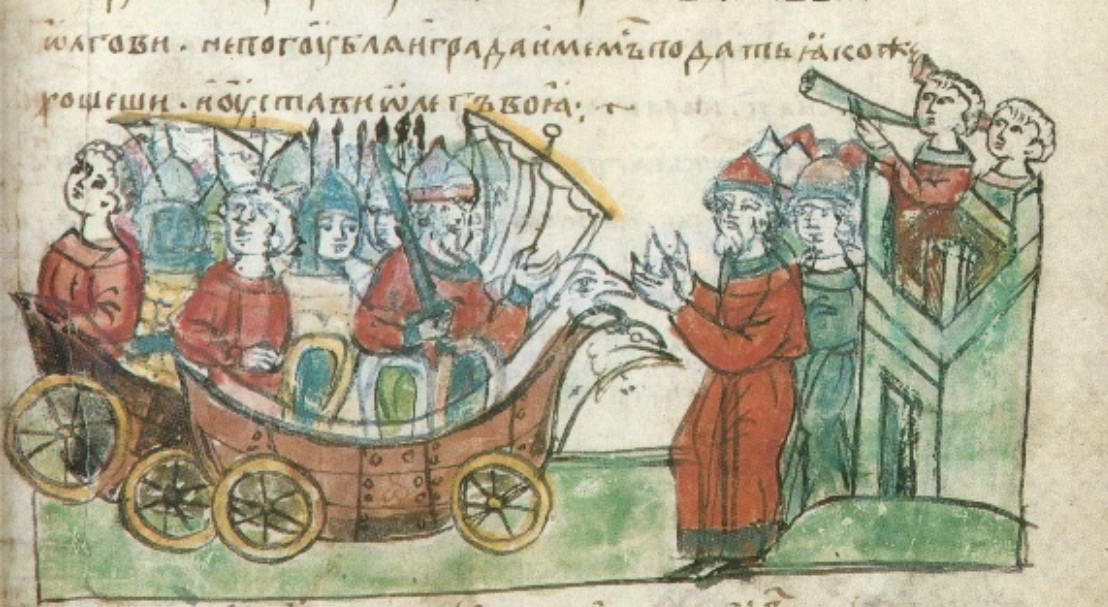
\includegraphics[width=\linewidth]{chast-volga/olg/kolesa.jpg}
\end{center}

Во время переговоров Греки поднесли Олегу и дружине его «брашно и вино», но Олег вылил питье на землю, вовремя поняв, что его хотят отравить. И своим людям приказал ничего от даров не есть и не пить. Убояшася Греци и реша: «несть се Олег, но святый Дмитрей, посланный на ны от бога». 

Не знаю, почему именно Дмитрий. Быть может Греки усмотрели сходство с сюжетом из жития Дмитрия Солунского, которого хотели отравить жалом скорпиона. Дмитрий перекрестил скорпиона, плюнул на него, и тот умер.

Зачем Олег привел с собой 2000 кораблей? Он решил наложить на Царьград дань по числу кораблей, 12 гривен на человека, из расчета, что в корабле «40 муж». Греки согласились и предложили заключить мир. Олег отступил от стен и послал в город, к царям Леону и Александру, послов: Карла, Фарлофа, Вельмуда, Рулава и Стемида (Корла, Форлофа, Велемудра). Летописи пересказывают договор, заключенный между Русью и Византией, местами приводя выдержки.

Условия мира таковы – кроме упомянутой дани, также и некие «уклады на Рускыя грады: первое на Киев, таже на Чернигов, на Переславль, на Полтеск, на Ростов, на Любеч и на прочаа городы, по тем бо городом седяху велиции князи, под Олгом суще». Я пытался разобраться в смысле «укладов» – что это, единоразовая ли дань городам, где у Олега наместники сидели, или постоянная, либо подарки – ибо сумма ведь не указана, сколько каждому городу. Историков кажется это не заботит, просто цитируют – да, мол, уклады. Татищев трактует уклады так – дань, платимая каждый год.

Еще о кораблях на колесах. Наука не располагает древнерусскими кораблями. Они все вроде бы сгнили! Где-то на Ладоге и в Новгороде впрочем нашли некие остатки, решив что это от «ладьи викингского типа». Никаких точных сведений о славянских судах того времени у нас нет. Может некоторые суда были изначально приспособлены к установке на колеса? Всё же корабль так удобнее тащить, нежели просто «волоком». 

Если у византийцев был «греческий огонь» – огнеметы, причем некоторые, судя по рисункам, весьма небольшие, размером с автомат Калашникова – то у Русов вполне могли быть колесные корабли. На рисунке в Радзивилловской летописи эти колеса вообще как на советских детских велосипедах – с толстыми спицами и шинами. 

Как вообще «тащили волоком»? С Рёриха повелось изображать это так: валят лес, тешут бревна, подкладывают их под корабль – эх ухнем – волочат по бревнам, потом бревна позади вынимают, впереди ими стелют, и корабль дальше толкают. Хорошо, а если леса нет? Или его не хватает на все корабли? А сколько нужно человекосил, чтобы перемещать корабли по бревнам?

Художник Васнецов нарисовал волок следующим образом – поставил корабль на колеса. Да, судно на колесах, и тащат его лошади. У Васнецова впрочем под судно подводится рама с колесами, и туда кладется судно.

Как выглядели волоки на самом деле, никто не знает. В Ремезовской летописи (17-18 века) есть миниатюра перемещения волоком, где Ермак переправляется через Уральские горы, возле Тагила. Под судном видны бревна, а спереди впряжены люди, и тянут. Играют ли бревна роль колес или перемещение осуществляется «рёриховским» способом – неведомо.

\begin{center}
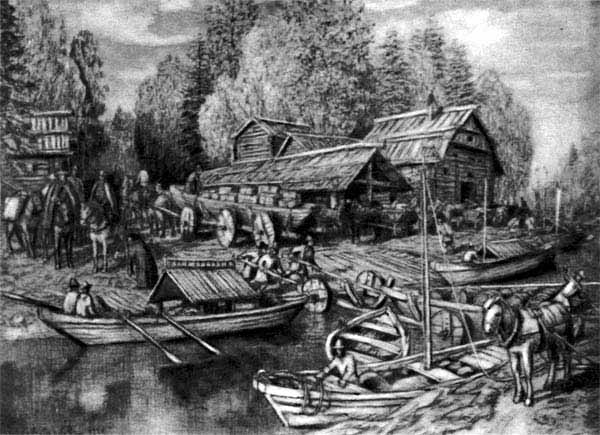
\includegraphics[width=\linewidth]{chast-volga/olg/volok.jpg}

\textit{А. М. Васнецов – «Волок Ламский».}
\end{center}

К вопросу о древних колёсах мы еще обратимся в этой книге далее, рассуждая о Трое. Вернемся к Олегу. 

Судна на колёсах упомянуты в летописи лишь в связи с Олегом, и вероятно, как нечто из ряда вон выходящее, ведь для осажденных царьградцев сие было устрашающей диковинкой. Напрашивается вывод, что такая технология была использована только Вещим Олегом – хотя, повторюсь, мы ничего не знаем об устройстве тогдашних судов, а из летописи неясно, как относится к наличию колес на кораблях сам летописец. Дивно ли ему?

Не могу удержаться еще от одного предположения – что колесный флот Олега был иллюзией. Ведь в бой эти странные корабли не вступили. На Руси такое называли отводом глаз. Согласно преданиям, сильно преуспел в подобном Яков Вильгельмович Брюс\footnote{Его подмосковная усадьба «Глинки» пронизана подземными ходами, что соединяли все постройки и уходили за пределы усадьбы черт знает куда. Вероятно, подземные ходы были здесь прежде, до водворения Брюса. Брюс занимался тут своими изысканиями.}, соратник Петра I, главный артиллерист России\footnote{Во многом благодаря отлично поставленному Брюсом артиллерийскому делу тогдашняя армия России одерживала победы в важных сражениях.}, знаток множества наук, почитавшийся в народе чародеем. Молва приписывает ему с Петром разговор, где царь предлагал Брюсу применять иллюзии на войне в качестве отвлекающего манёвра, однако Брюс отказался, возразив, что так нечестно. 

Что же дальше? Олег заключает первый по летописному счету мир с Греками. Царьград будет платить дань, а Олег в случае чего пособит военной силой. По некоторым спискам, вместе с Олегом – Игорь. Олег в знак победы прибивает на Галатских воротах города щит, не то Игоря, не то свой (польский историк Стрыйковский говорил, что видел этот щит своими глазами в 1575 году). Затем возвращается в Киев.

Проходит несколько лет, в которые летопись отмечает одно лишь важное события – явление звезды копейного образа, в 911 году.

В 912 году Олег вторично посылает в Царьград послов. Сохранился текст мирного договора, с датой, согласно тексту изданий ПСРЛ – 2 сентября, недели 15, года 6420. Назойливо напомню – всего этого нет в дошедшей до нас Лаврентьевской летописи, изъято, вырвано. Что-то происходящее в эти годы там было изложено, но сколь совпадало оно с содержимым Ипатьевского и Радзивилловского списков?

Договор. В нем обращаются к самодержцам Льву, Александру и Константину. Послов больше, частью это уже знакомые имена: Карлы, Инегелд, Фарлоф, Веремуд, Рулав, Гуды, Руалд, Карн, Фрелав, Руар, Актеву, Труан, Лидул, Фост, Стемид.

Осенью 912 года, по возвращении послов, Олег вспоминает коня своего. По Ипатьевскому списку Повести временных лет этот сюжет передан сокращенно, без свадебного пира по поводу бракосочетания Игоря и Ольги, без обещания Олега вознаградить того, кто предречет ему смерть, без умерщвления волхвов:

\begin{quotation}
И живяше Олег, мир имея к всем странам, княжа в Киеве. И приспе осень, и помяну Олег конь свой, иже бе поставил кормити, не вседати на нь. Бе бо преже въпрошал волъхвов и кудесник: «От чего ми есть умьрети?». 

И рече ему один кудесник: «Княже! Конь, егоже любиши и ездиши на нем, от того ти умрети». Олег же приимъ в уме, си рече: «Николи же всяду на конь, ни вижю его боле того». И повеле кормити й и не водити его к нему, и пребыв неколко лет не дея его, дондеже и на грекы иде. 

И пришедшю ему к Киеву и пребысть 4 лета, на 5 лето помяну конь свой, от негоже бяху рекъли волъсви умрети Ольгови. И призва старейшину конюхом, ркя: «Кде есть конь мой, егоже бехъ поставилъ кормити и блюсти его?». Он же рече: «Умерл есть».

Олег же посмеяся и укори кудесника, ркя: «То ть неправо молвять волъсви, но все то лъжа есть: конь умерл, а я жив». И повеле оседлати конь: «Да ть вижю кости его». И приеха на место, идеже бяху лежаще кости его голы и лоб гол, и слез с коня, посмеяся, ркя: «От сего ли лъба смерть мне взяти?» И въступи ногою на лоб, и выникнучи змея и уклюну и в ногу. И с того разболевся, умьре. И плакашася по нем вси людие плачем великом, и несоша и, и погребоша и на горе, иже глаголеться Щековица; есть же могила его до сего дни, словеть могила Олгова. И бысть всех лет его княжения 33.
\end{quotation}

То бишь при Несторе, по его словам, могила Олгова слыла на Щековице. Что за могила? Вероятно, курган – ведь Олег был язычником. Синопсис подтверждает: «Погребен же бысть на горе Шковице по обычаю поганскому».

В списках находим расширенный вариант предания:

\begin{quotation}
И по сем женися князь Игорь Рюрикович во Плескове, поя за себя княжну, именем Олгу, дщерь князя Тмутаракана Половецкаго.

И нача Олг князь со Игорем веселитися, творяще пирования веселого много, и егда Олг князь на веселие\footnote{На свадьбе.} рече боляром своим о себе, яко аз новый есмь царь александр макидонский мудростию и храбростию надеяся обладати всем светом; да еще могл кто угонуть\footnote{Угадать.}, от чего мне будет смерть, тогда бы тому много имения дал.

И тогда прилучися у Олга князя два мужа кудесника и рекоша к нему: то, господине, мы ведуем гораздо, от чего тебе, княже, хочеть смерть бы: есть, господине, у тебя любимый конь твои, от того тебе будет смерть.

Князь же Олег не полюби тои смерти и возвещая своим боляром на сих кудесниках и рече: послушайте вси, да скажю вам, како сии мужие предрекли мне смерть злую, яко от лучшаго коня мне умрети. 

И по сем вопроси кудесников: и вам от чего будет смерть?

Они же к нему рекоша: тебе, княже, от коня, а нам от тебя смерть будет.

И рече князь Олг: то будет по моей воли, и вас погубить не велю и на коне своем ездили не хощу, да не велю его водить перед себя. Да егда то будет, седмь лет минется\footnote{В этом разговоре Вещего Олега с кудесниками усматриваю соревнование в пророчествах самого волхва-Олега с другими волхвами.}.

На осмое лето на пиру воспомянул Олг князь конь своий любимый и вопроси конюшего своего о коней? «где тот конь мой любимый, от которого мне прорекли кудесники, что умрети мне от него?».

Рече же ко Олгу конюшей его: господине княже, уже три годы минулось, как тот конь твой любимый умре.

Князь же о сем посмеявся не мало и рече кудесником: ту суть неправии ваши речи.

И тако князь Олг повеле их обесити на древе, и сам князь вседе на ин конь и поиде з боляры своими, и ехавше ему путем, и обрете окрест града кость лежащу, главу коневу, и рече конюшей ко олгу князю: вот, господине княже, глава твоего любимаго коня.

И князь нача смеятися и рече: брате мои и друже, и те кудесники осуждены на смерть за то, что мне от него прорекли смерть.

И сам князь Олг сниде с коня своего и ступи ногою на лоб, на сухую главу коневу, и рече глумяся: с от тебе мне прорекли умрети!

И выкинулася змия из главы тоя великая и тако ужали князя Олга за ногу, и от того разболеша и умре.

И тако людие начаша тужити о кудесниках, что их князь осуди без вины на смерть лютую.
\end{quotation}

Этот стройный рассказ в «общепринятых» списках сокращен, а части его переставлены во времени. История с пророчеством всплывает кстати, когда Олег вдруг припоминает любимого коня...

Любопытно – будучи христианским монахом, Нестор ранее дал отрицательную оценку тому, что Олега называли Вещим, то бишь провидцем. Мол, по темноте поганства своего, люди сочли Олега вещим. Здесь же Нестор (ли?), не поморщившись, описывает воплощение пророчества, данного кудесниками, в жизнь. Да еще пускается в рассуждения: «се же дивно есть, яко от волхствования сбывается чародейством» и далее дает примеры успешного исполнения пророчеств, изреченных волхвами.

Для полноты картины снова обратимся к книжке Гилярова, поглядим на варианты этого события в списках.

По одним, Олег повелел коня уморить. По другим – таки кормить, но сам видеть его не хотел, ездить на нем не ездил. Олег также приказал уморить волхва, который предрек ему смерть. Один список уточняет, что Олег приказал отвести коня далеко в поле и отрубить голову. А новгородцы пишут, что Олег после Киева отправился в Новгород, потом в Ладогу, и там-то, когда отправился он за море, его укусила змея, и что могила Олега находится в Ладоге. Теперь это поселок Старая Ладога, Ленинградской области.

В самом деле, там показывают туристам местную Олегову могилу – курган со срезанной верхушкой на берегу реки Волхов, метров десяти высотой и около тридцати в диаметре.

Вспоминается Чингисхан – когда он умер, сыновья возвели восемь могил в разных местах, дабы сбить с толку тех, кто захочет побеспокоить прах. До гибели своей (упал с лошади и занемог) Чингисхан приказал о будущей смерти никому не говорить, не оплакивать его, чтобы враги не проведали. Мертвое тело везли,  нетленности ради, в бочке с медом – к некой горе. До сих пор ищут.

Археологам известны кенотафы – ложные захоронения. Были и пустые древнерусские курганы. Погодите, погодите! Вне ереси о Киеве, по которой Олег не только остался жив, но здравствовал в образе княгини Ольги, у нас есть две могилы Олега. Обе связаны с летописным преданием. Одна могила должна быть пустой. А если обе?

Могила Олгова на Щекавице. А где похоронена княгиня Ольга? Неведомо.

Про курган Олегова могила в Старой Ладоге. Археологи его повредили, раньше он был на четыре метра выше. Олегова могила – лишь один из ряда шестерых курганов вдоль берега реки Волхов. На восточной окраине поселка есть еще один, а эти шесть – в полукилометре на северо-восток.

Название кургана Олеговой могилы в научной литературе – «Полая сопка», «сопка Ходаковского». Еще в 1820 году на ней проводил раскопки Зориан Доленга-Ходаковский, он же Адам Чарноцкий. Исследовав примерно треть кургана, археолог нашел немного – несколько сожженных костей, копейный наконечник 8-9 веков, угли, кусок железа, «похожий на задвижку в замке».

Внутри кургана прорыт подземный ход, ведущий в разветвленные пещеры. В окрестностях Старой Ладоги существует две пещерных системы, или просто пещеры – Староладожская\footnote{Вход находится по координатам 60°0'23"N 32°17'42"E – 64 метра на юго-восток от церкви рождества Иоанна Предтечи, в нижней части Малышевой горы.} и Таничкина (Староладожская-2, Макароны).

Староладожская пещера – со сводами и колоннами, местами разрушена, местами затоплена, загажена надписями. Общая длина её изученной части – 410 метров. Между переходами есть залы высотой три, иногда до четырех метров. В западном углу имеется родник. Будто бы раньше это была естественная пещера, а потом, в конце 19-го и начале 20 веков, здесь добывали кварцевый песок для стекольного завода, что пещеру преобразило. Как именно? Есть мнение, что эти залы и колонны сделали рабочие. Современники тех земляных работ ничего не расскажут. А в 1950 году вход в пещеру завалили, чтобы никто не ходил, ибо там пропало двое людей. Местные тогда считали, что пещерные ходы тянутся на 15 километров.

Таничкина пещера\footnote{60°0'44"N 32°18'46"E} имеет два входа на обрывистом берегу Волхова, примерно в 330 метрах к востоку от самого восточного кургана. Длина Таничкиной пещеры около 7,5 километров. Коридоры – не залы – там низкие. Ученые тоже считают, мол, как и Староладожская, пещера образовалась при отработке пласта белых кварцевых песчаников. 

При этом ученые дают пещерам возраст то 150 лет, то отодвигают в более глубокое прошлое. Я же думаю, что пещеры существовали до того, как местное население стало добывать в них песок. 

Но о курганах! В 19 веке местные предания о том, что в кургане на берегу Волхова похоронен именно Олег, не записаны. Это археологи предположили Олегову могилу сначала в одном кургане, а потом в другом – который с легкой руки Н. Е. Бранденбурга и Г. С. Лебедева и прослыл под таким именем. Местные еще в начале 20 века называли курганы просто – сопки. Ходило также смутное предание, что в них либо в Новгороде погребен Рюрик.

А вот киевская Олегова могила на Щекавице или около – напротив, известна была еще летописцам, и предание непрерывно из века в век сохранялось в народе. Подробно об этом месте я рассказал в главе про Щекавицу. Но как бы ни было, существуют летописные списки, указывающие на гибель Олега в Ладоге.

%Про Олегову могилу на Щекавице не могу понять. Либо считалось, что там похоронен Вещий Олег (ложная смерть, пустой курган), либо Вольга как княгиня Ольга. В летописи сказано – могила Олгова, а это можно трактовать как угодно. Олгова – и Олега, Олгова – и Ольгина.

Со смертью Вещего Олега еще странность. Татищев откуда-то выписал:

\begin{quotation}
[...] разболеся Олег умре, и плакаша по нем людие вси плачем великим. Вынесши же погребоша его на горе, яже глаголется Щековица, где есть могила его, и до сего дни слывет могила Олгова, и бысть в сех лет княжения его 33. Сея же зимы погоре небо, и столбы огненные ходили от Руси ко Греции сражающиеся. Олег же принесе жертвы многи умилостивляя богов своих нечистых.
\end{quotation}

Допустим, у Татищева надежный источник, хотя слог его кажется мне близким к петровской эпохе.

Что за столбы огненные? «Звезда копейного образа» из другого списка, за 911 год? Или другое явление? Описание всё же отличается от копейного образа. Столбы огненные, да еще сражающиеся. Олег на это приносит жертву языческим богам.

Вспомним пророчество кудесников о смерти Вещего Олега. Я не верю в чудеса. Пророчества сбываются, если им помогают воплотиться в жизнь.

Вольга заранее продумал, когда «умрет» в качестве Вещего Олега. Заранее подготовил легенду, пророчество – так, чтобы это стало известно народу. Теперь чтобы исчезнуть, ему оставалось сказать, что уезжает на останки коня любимого поглядеть. «И абие изыде из главы из коневы, из сухия кости змий, и уязви Ольга в ногу по словеси волхвов его, емуже предрекоша умрети от своего любимого коня. И оттоле разболеся и умре».

Если только всё это не басня, выдуманная вместо листов, изъятых из Лаврентьевской летописи.

%Тайной остаются сведения о десятилетней девочке, которую Олег выбрал Игорю в жены и нарёк, по своему имени, Олгой. Управляемый, безвольный ребенок – из простой семьи варягов (по одному из списков) – должен быть повзрослеть точно ко времени «ухода» Вещего Олега. Вольга не собирался не только умирать, но и привыкать к другому имени!

%Что случилось с девочкой потом? Она должна была исчезнуть. А может не было никакой девочки, но тогда Вольге пришлось бы какое-то время изображать двух разных людей. По одним спискам – около 10 лет, по другим – в течении года. Сложно разобраться, как было на самом деле. Судим ведь по летописным сведениям. А вдруг там выдумка? А вдруг «смерть» Олега – понятие образное, как, допустим, уходящий в монастырь человек умирает для «мира»? Смену образа, отказ от себя былого, властитель Вольга мог обставить торжественно.

Вещий Олег уходит со сцены. Накануне своего ухода, зимой, если верить источнику Татищева, Олег приносит «жертвы многи» после странных явлений в небе. Думаю, неспроста именно затем был заключен второй договор с Греками (куда из Руси ходили упомянутые огненные столбы), и Олег, как бы завершив все насущные дела, прекращает быть князем Олегом и принимает образ княгини Ольги.

Если только это разделение одной личности на две не «книжное», не возникшее позже в летописях.